\documentclass[a4paper,10pt,twocolumn]{scrartcl} %Koma-Skript-Äquivalent zu "article"

%Von Elias entfernte Packages: inputenc, scrpage2
%\usepackage{scrpage2}          %ermöglicht änderung der Kopf-/Fußzeile


%\usepackage{german}            % Entfernt, um deutsche Überschriften zu vermeiden
\usepackage[english]{babel}    % Setzt die Sprache auf Englisch
%\usepackage[latin1]{inputenc}  %man kann Sonderzeiche wie ü,ö usw direkt eingeben
\usepackage{amsmath}           %macht
\usepackage{amsfonts}          %       Mathe
\usepackage{amssymb}           %              mächtiger
\usepackage{graphicx}          %erlaubt Graphiken einzubinden (.eps für dvi und ps sowie .jpg für pdf)
\usepackage[T1]{fontenc}       %Zeichenbelegung der verwendeten Schrift
\usepackage{ae}                %macht schöneres ß
\usepackage{typearea}	         %ermöglicht änderung des Seitenspiegels
\usepackage{lastpage}          %lässt auf die Seienanzahl zugreifen
\usepackage[margin=10pt,font=small,labelfont=bf]{caption} %macht die Bildbeschriftungen richtig
\usepackage{hyperref}          % Fügt Unterstützung für Referenzen und Links hinzu
\typearea{16}                  %stellt Seitenspiegel ein
\columnsep25pt								 %definiert Breite zwischen den zwei Spalten von \twocolumns

\pretolerance=10000 % Erhöht die Toleranz für Textaufteilung
\hbadness=10000     % Unterdrückt Underfull \hbox-Warnungen

\renewcommand{\pnumfont}{%     %ändert die Schriftart der Seitennummerierung
\normalfont\rmfamily\slshape}  %ändert die Schriftart der Seitennummerierung 

% Beispiel für ein Makro
\newcommand{\platzhalter}{??Platzhalter??}

\newcommand{\sigmaXXBzero42}{\left(5.40 \pm 0.11\right) \cdot 10^{-3}\,\text{S}}
\newcommand{\sigmaXXBzero3}{\left(5.39 \pm 0.11\right) \cdot 10^{-3}\,\text{S}}
\newcommand{\sigmaXXBzero21}{\left(5.39 \pm 0.11\right) \cdot 10^{-3}\,\text{S}}
\newcommand{\sigmaXXBzero14}{\left(5.38 \pm 0.11\right) \cdot 10^{-3}\,\text{S}}
\newcommand{\RHall42}{\left(2.8478 \pm 0.0012\right) \cdot 10^{3}\,\text{\Omega\,\text{m}}}
\newcommand{\RHall3}{\left(2.8488 \pm 0.0014\right) \cdot 10^{3}\,\text{\Omega\,\text{m}}}
\newcommand{\RHall21}{\left(2.8506 \pm 0.0012\right) \cdot 10^{3}\,\text{\Omega\,\text{m}}}
\newcommand{\RHall14}{\left(2.8513 \pm 0.0013\right) \cdot 10^{3}\,\text{\Omega\,\text{m}}}
\newcommand{\my42}{\left(1.537 \pm 0.031\right) \cdot 10^{1}\,\text{\text{m}^2/\text{Vs}}}
\newcommand{\my3}{\left(1.536 \pm 0.031\right) \cdot 10^{1}\,\text{\text{m}^2/\text{Vs}}}
\newcommand{\my21}{\left(1.536 \pm 0.031\right) \cdot 10^{1}\,\text{\text{m}^2/\text{Vs}}}
\newcommand{\my14}{\left(1.535 \pm 0.031\right) \cdot 10^{1}\,\text{\text{m}^2/\text{Vs}}}
\newcommand{\nZwei42}{\left(2.1176 \pm 0.0076}
\newcommand{\nZwei3}{\left(2.1139 \pm 0.0076}
\newcommand{\nZwei21}{\left(2.1018 \pm 0.0076}
\newcommand{\nZwei14}{\left(2.0958 \pm 0.0076}
\newcommand{\nEins42}{\left(2.19167 \pm 0.00095}
\newcommand{\nEins3}{\left(2.1909 \pm 0.0011}
\newcommand{\nEins21}{\left(2.18957 \pm 0.00094}
\newcommand{\nEins14}{\left(2.18901 \pm 0.00099}
 % Korrekte Einbindung der Datei macros.tex


\begin{document}

% Titel und Abstract über beide Spalten
\twocolumn[{\csname @twocolumnfalse\endcsname
\titlehead{
    \begin{tabular*}{\textwidth}[]{@{\extracolsep{\fill}}lr}
    Supervisor: Dr. Piatrusha & \today\\ % \today zeigt jetzt das Datum auf Englisch an
    \end{tabular*}
    }
\title{Quantum Hall effect in a two-dimensional electron gas}
\author{Lukas Hein, Elias Schwarzkopf}
\date{}
\maketitle
\vspace{-8ex}
\begin{abstract}                                                %Beginn des Abstracts
    \noindent Lorem ipsum dolor sit amet, consetetur sadipscing elitr, 
    sed diam nonumy eirmod tempor invidunt ut labore et dolore magna aliquyam erat, 
    sed diam voluptua. At vero eos et accusam et justo duo dolores et ea rebum. 
    Stet clita kasd gubergren, no sea takimata sanctus est Lorem ipsum dolor sit amet. 
    Lorem ipsum dolor sit amet, consetetur sadipscing elitr, sed diam nonumy eirmod tempor invidunt ut 
    labore et dolore magna aliquyam erat, sed diam voluptua. At vero eos et accusam et justo duo dolores et ea rebum. 
    Stet clita kasd gubergren, no sea takimata sanctus est Lorem ipsum dolor sit amet.
    \\
    \\ 
    Experiment:\,April 8, 2025\\       %Datum ändern!
    Submission: \today                 %Datum ändern!
    \\ 
    \\ 
\end{abstract} % Abstract bleibt über beide Spalten
\vspace{-6ex} % Reduziert den Abstand nach dem Abstract
}]

\section{Introduction}
The Quantum Hall Effect (QHE) is one of the simplest ways to measure the ratio between Planck's constant 
and the elementary charge. In 1985 Klaus von Klitzing discovered the QHE in a two-dimensional system which
desribes the quantization of the transverse resistivity $\rho_\text{xy}$ in multiples of $h/e^2$ \cite{Nobelpreis}, later called the von 
Klitzing constant.
This made it possible to define a new resistivity standard that depends only on fundamental constants. 
In the following sections, the QHE and it's related properties are determined and discussed. 
The main part of this paper is the analysis of the transverse resistivity and the appearance of the Hall plateaus.
The carrier density is determined by different methods and compared. 
The cyclotron mass, Fermi energy and Fermi velocity are also calculated.
Finally, we will investigate whether a spin-orbit coupling effect can be observed 
in the system and search for plateaus of the fractional quantum Hall effect.\\


\section{Set-Up}\label{sec:setup}
For the study of the QHE a two-dimensional or quasi two-dimensional system is needed.
In this experiment a quantum well is created by confining electrons in a thin layer of HgTe between
two layers of HgCdTe. Because of the smaller bandgap of HgTe compared to HgCdTe a quantum well is formed. 
At low temperatures, all electrons are located in the lowest energy level of the 
two dimensional quantum well. This creates a confinement in the layer stacking direction.
Inside the quantum film of HgTe, the electrons form a two-dimensional electron gas (2DEG) with high mobility.
The sample is designed in a common Hall bar geometry,
with $8$ contacts on the edges with a additional pair for the gate voltage (see fig.\,\ref{fig:HallBar}).
The gate voltage is set to $V_\text g = -0.25V$ if not stated differently.
\begin{figure}[h]
    \centering
    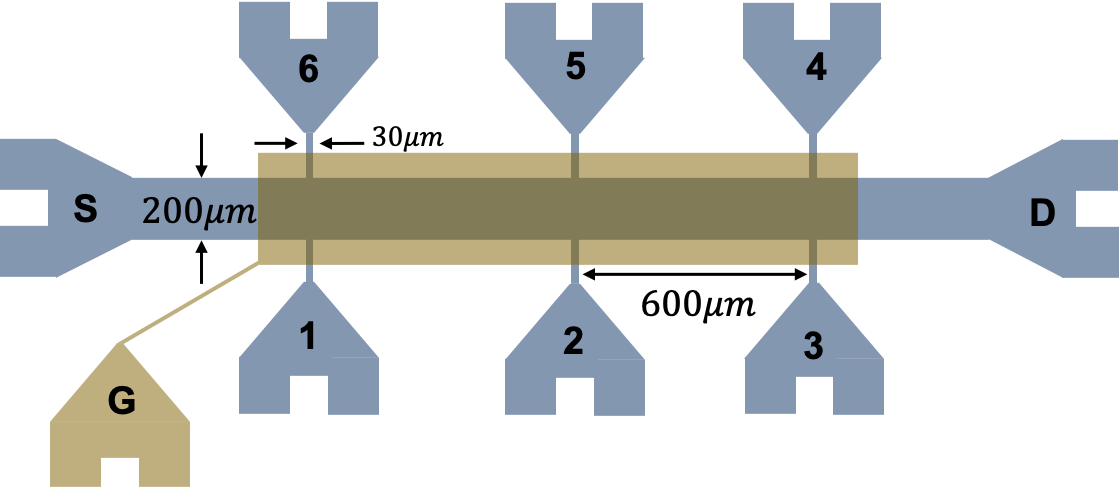
\includegraphics[width=0.45\textwidth]{../Images/HallBar.png}
    \caption{Schematic of the Hall bar geometry. The contacts are labeled with "S" for source, "D" for drain,
    "G" for gate. Contacts $4$ and $6$ are used for the measurement of the longitudinal resistance 
    and contacts $3$ and $4$ are used for the measurement of the transversal resistance.}
    \label{fig:HallBar}
\end{figure}
An AC voltage is applied between source and drain to control the longitudinal current $I$
flowing through the sample. $I$ can be measured via the voltage drop $U_\text{I}$ over a known resistor $(R_\text{S}=4.982\pm0.0005)\,\text{k}\Omega$, 
which is connected in series to the source contact. $U_\text{I}$ is measured with a Lock In amplifier 
\emph{Stanford Research Systems SR510}. Contacts $3$ and $4$ are used to measure the hall voltage $U_\text{Hall}$, which
is measured with a second Lock In amplifier of the same type. Contacts $4$ and $6$ are used to measure
the longitudinal Voltage $U_\text{xx}$, which is measured with a third Lock In amplifier \emph{Stanford Research Systems SR530}.
All Lock In amplifiers use a phase sensitive amplification approach by filtering the the noise through multiplying the signal
with a $13\,\text{Hz}$ reference signal. Moreover, the data is integrated over a period of $3\,\text{s}$ and measured with a sensitivity of $1\,\text{mV}$.
The gain accuracy is $1\%$.
The hall bar sample has a width of $200\,\mu\text{m}$ and a length of $1.2\,\text{mm}$, which can be seen in fig.\,\ref{fig:HallBar}.
For observation of the hall effect, a magnetic field $B$ is applied perpendicular to the plane of the sample.
The magnetic field is generated by a superconducting NbTi solenoid, which is cooled with liquid helium and can
be precisely controlled by the current flowing through the magnet. The flux density $B$ is read out as a voltage
$U_\text{B}$ with $U_\text{B}=10\,\text{V}$ corresponding to $9\,\text{T}$. 
The Hall bar is placed inside a variable temperature insert (VTI), 
which allows to cool down the sample by evaporating liquid He at different pressures. 
The measurements are taken at the temperatures $\csname tempFor4.2K\endcsname$, 
$\csname tempFor3K\endcsname$, $\csname tempFor2.1K\endcsname$, $\csname tempFor1.4K\endcsname$, which will be referred as the goal temperatures
$4.2K$, $3K$, $2.1K$ and $1.4K$ respectively.
The temperature of the sample is measured via the voltage drop over a $Alan Bradley$ resistor 
$R_\text{AB}=100\,\Omega$ using a \emph{Keithley 160B} digital multimeter and a constant current of $10\mu\text{m}$.
Acting as a resistive thermometer the carbon resistor is located with the sample inside the VTI and is calibrated for the used temperature range.
The conversion of Voltage to Temperature is done with the calibration table \cite{ExperimentDescription}.
The temperatures could not be stabilized perfectly, so the mean temperature between the beginning and the end of the measurement is taken.
While the magnetic field is turned on, the temperature could not be measured, since the resistor is dependent on the magnetic field.
Since the resistor is not exactly positioned at the Hall bar and its error is not known, the error in temperature is estimated to be $1\%$.
If half of the drift in temperature is larger, half of the drift is used as error. 



\input{experiment}
\section{Summary}

In this work, the Quantum Hall Effect (QHE) was investigated in a two-dimensional electron system 
at low temperatures and high magnetic fields. 
The QHE provides a precise method to measure the ratio of Planck's constant $h$ to the elementary charge $e$,
leading to the determination of the von Klitzing constant $R_\text{K}$. Our measurements confirm the 
quantization of the Hall resistivity $\rho_\text{xy}$ in multiples of $h/e^2$, with the experimentally 
determined $R_\text{K}$ values agreeing with the exact value of $R_\text{K, exact} = \csname Klitzing1.4K\endcsname\,\text{k}\Omega$ 
within experimental uncertainties.
The charge carrier density $n$ was determined using three different methods: 
the classical Hall effect, the quantum Hall plateaus, and the Shubnikov-de Haas oscillations. 
The results were consistent across methods, with $n$ values in the range of $\csname nEins1.4K\endcsname \cdot 10^{15}\,\text{m}^{-2}$, 
showing a slight temperature dependence.
The cyclotron mass $m_\text{c}$ was calculated from the temperature dependence 
of the oscillation amplitudes in the longitudinal conductivity $\sigma_\text{xx}$. 
The determined values, $m_\text{c} = (\csname cyclotron15\endcsname)\cdot 10^{-2}m_\text{e}$ for the $1.4\,\text{K}$ and $3\,\text{K}$ 
pair and $m_\text{c} = (\csname cyclotron21\endcsname)\cdot 10^{-2}m_\text{e}$ for the $2.1\,\text{K}$ and $4.2\,\text{K}$ pair, 
are in good agreement with literature values.
Additionally, the Fermi wave vector $k_\text{F}$, Fermi energy $E_\text{F}$, and Fermi velocity $v_\text{F}$ 
were calculated assuming a parabolic energy dispersion. For $T = 4.2\,\text{K}$, 
the results were $k_\text{F} = (\csname kFermi4.2K\endcsname) \cdot 10^{8}\,\text{m}^{-1}$, $E_\text{F} = (\csname EFermi4.2K\endcsname)\cdot 10^{-2}\,\text{eV}$, 
and $v_\text{F} = (\csname vFermi4.2K\endcsname) \cdot 10^{5}\,\text{m/s}$. 
These values highlight the low-energy nature of the system and the necessity of 
low temperatures to maintain the two-dimensional confinement.
No evidence of the fractional Quantum Hall Effect (FQHE) was observed in the accessible magnetic field range. 
The absence of fractional plateaus and corresponding longitudinal resistivity peaks suggests that higher magnetic 
fields are required to observe this phenomenon.
In conclusion, the experimental results confirm the fundamental properties of the Quantum Hall Effect 
and provide insights into the electronic properties of the system, including charge carrier density, 
cyclotron mass, and Fermi parameters. The findings are consistent with theoretical predictions and 
highlight the precision of the QHE as a tool for fundamental physics and metrology.

\begin{thebibliography}{99}
    \bibitem{Nobelpreis} K. von Klitzing, G. Dorda, and M. Pepper, \emph{New Method for High-Accuracy
    Resistance Standard Based on Quantized Hall Resistance}, Phys. Rev. Lett. \textbf{45}, 494 (1980).
    \bibitem{ExperimentDescription} ja kommt noch

    \bibitem{klitzing}CODATA. (2018). CODATA recommended values of the fundamental physical constants: 
    2018. NIST Physical Measurement Laboratory.
    https://physics.nist.gov/cgi-bin/cuu/Value?rk



\end{thebibliography}



 % Manuelle Bibliographie einfügen
\end{document}
